\documentclass[tikz, border=2pt]{standalone}
\usepackage{amsmath}

\begin{document}
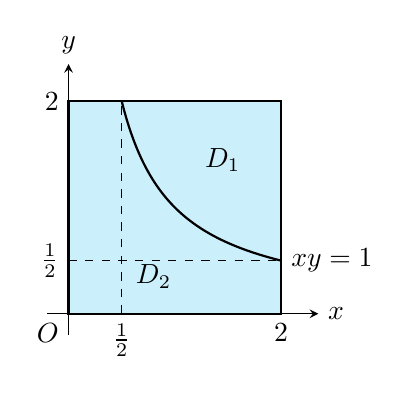
\begin{tikzpicture}[scale=1.35, >=stealth]
    % 填充积分区域 D
    \fill[cyan!20] (0,0) rectangle (2,2);

    % 画坐标轴
    \draw[->] (-0.2,0) -- (2.35,0) node[right] {$x$};
    \draw[->] (0,-0.2) -- (0,2.35) node[above] {$y$};

    % 画正方形边界
    \draw[thick] (0,0) rectangle (2,2);

    % 画分界曲线 xy=1
    \draw[thick, domain=0.5:2, samples=100] plot (\x,{1/\x}) node[right] {$xy=1$};

    % 画辅助线
    \draw[dashed] (0.5,0) -- (0.5,2);
    \draw[dashed] (0,0.5) -- (2,0.5);

    % 标注关键坐标点
    \node[below] at (0.5,0) {$\frac12$};
    \node[below] at (2,0) {$2$};
    \node[left] at (0,0.5) {$\frac12$};
    \node[left] at (0,2) {$2$};
    \node[below left] at (0,0) {$O$};

    % 标注区域
    \node at (1.45,1.45) {$D_1$};
    \node at (0.8,0.35) {$D_2$};
\end{tikzpicture}
\end{document}
